\documentclass{article}
\usepackage{fullpage}

\usepackage{tikz}
\usetikzlibrary {datavisualization.formats.functions}

\pagestyle{empty}

\begin{document}
\setlength{\parindent}{0pt}
\begin{center}
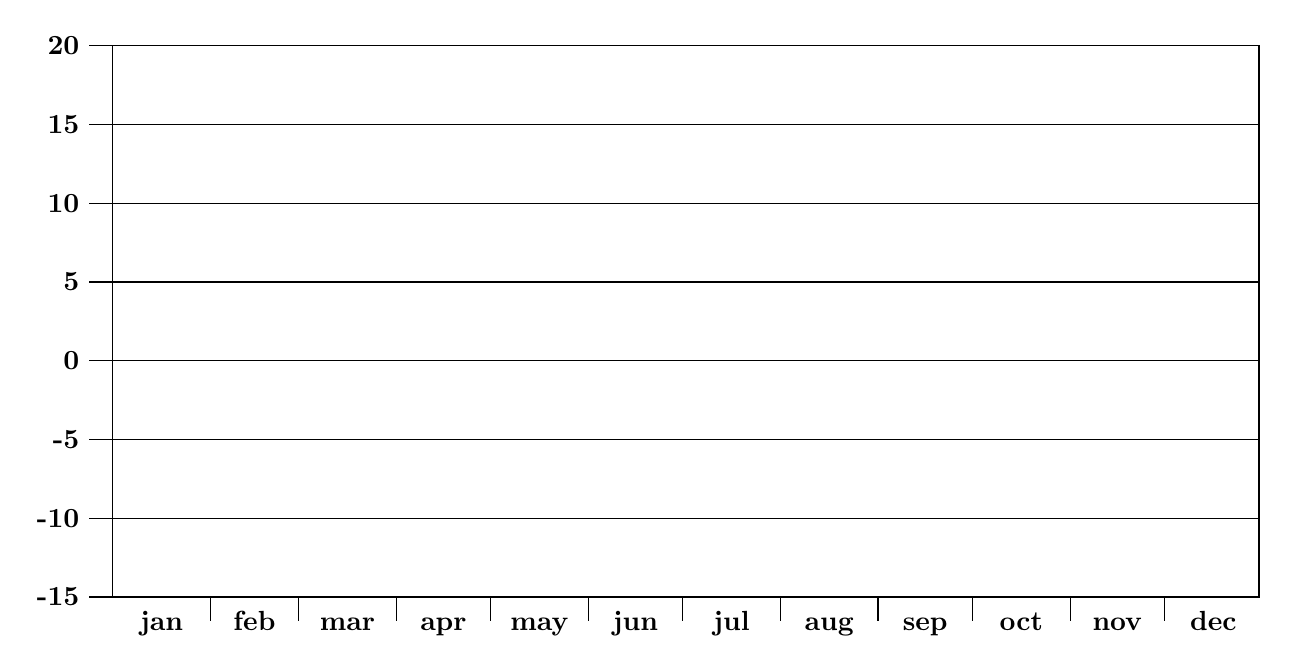
\begin{tikzpicture}[x=0.04cm,y=0.2cm]
  \draw[very thick] plot[smooth] file {eot.txt};
  \draw (0,-15) rectangle (364,20);
  \foreach \i in {-15,-10,...,20} {
    \draw (364,\i) -- (0,\i);
    \draw (0,\i) -- +(-3mm,0) node[left]{\textbf{\i}};
  }

  \foreach \i in {31,59,90,120,151,181,212,243,273,304,334} {
    \draw (\i,-15) -- +(0,-3mm);
  }

  \path (0,-15) {\foreach \i/\month in {31/jan,59/feb,90/mar,120/apr,151/may,181/jun,212/jul,243/aug,273/sep,304/oct,334/nov,365/dec} {-- node[below=3mm]{\textbf{\smash{\month}}} (\i,-15)}};
  %\draw[thin] (0,-17.4) -- +(365,0);


  %node[below] {\small aaa} 

\end{tikzpicture}
\end{center}

\newpage
\begin{center}
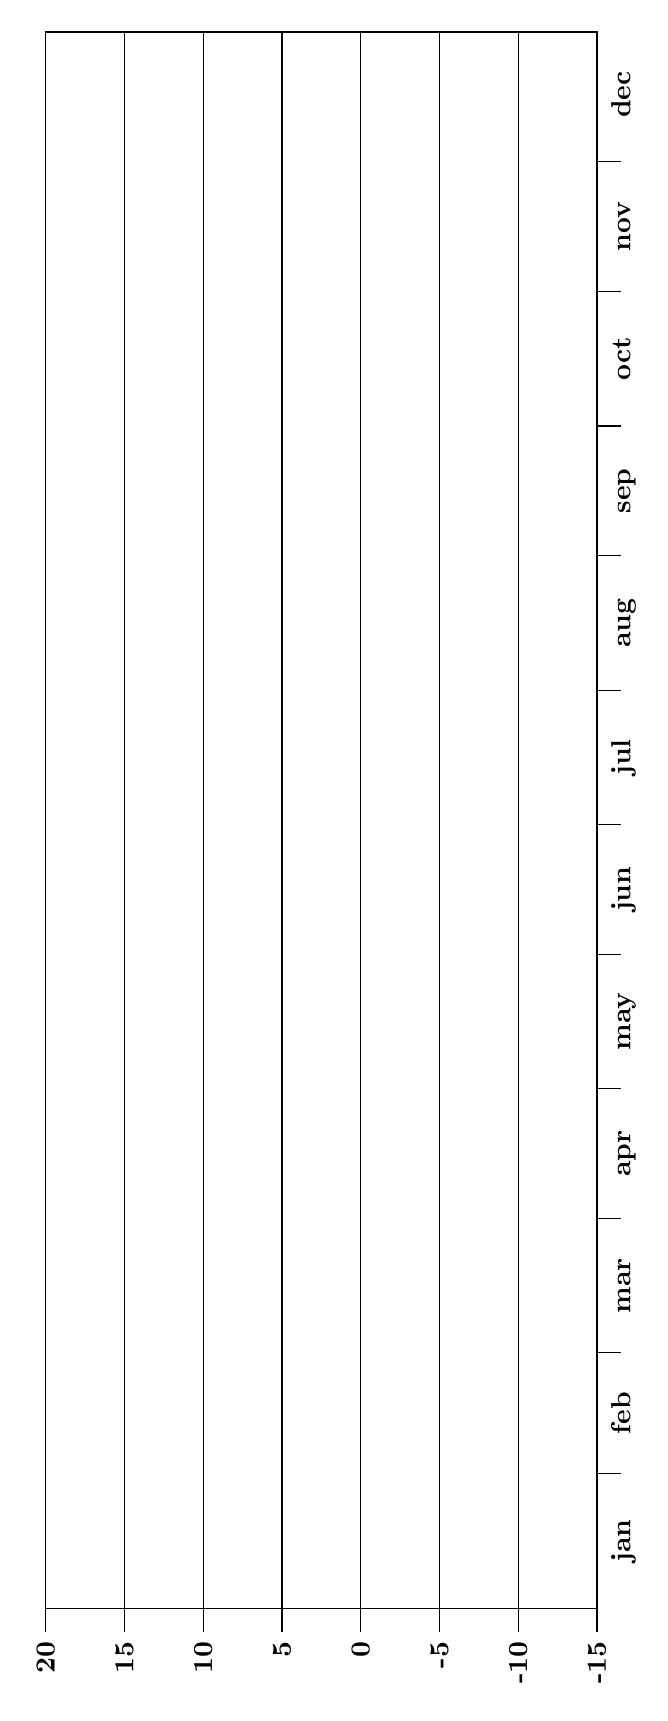
\begin{tikzpicture}[x=0.055cm,y=0.2cm]
\begin{scope}[rotate=90]
  \draw[very thick] plot[smooth] file {eot.txt};
  \draw (0,-15) rectangle (364,20);
  \foreach \i in {-15,-10,...,20} {
    \draw (364,\i) -- (0,\i);
    \draw (0,\i) -- +(-3mm,0) node[rotate=90,anchor=center,left]
    {\textbf{\i}};
  }

  \foreach \i in {31,59,90,120,151,181,212,243,273,304,334} {
    \draw (\i,-15) -- +(0,-3mm);
  }

  \path (0,-15) {\foreach \i/\month in {31/jan,59/feb,90/mar,120/apr,151/may,181/jun,212/jul,243/aug,273/sep,304/oct,334/nov,365/dec} {-- node[anchor=center,rotate=90,below=3mm]{\textbf{\smash{\month}}} (\i,-15)}};
  %\draw[thin] (0,-17.4) -- +(365,0);


  %node[below] {\small aaa} 
\end{scope}
\end{tikzpicture}
\end{center}

\end{document}
